\newpage
\section{Sensor}
\fxnote{skriv noget intro}


\subsection{1-Wire}
%https://www.maximintegrated.com/en/products/digital/one-wire.html
Sensoren benytter en 1-Wire forbindelse til at kommunikere med mikroprocessoren. 1-Wire er en teknologi hvor en  enkelt serial forbindelse fungere som data forbindelse i begge retninger. 

Dette gøres ved at forbinde dataforbindelsen på sensoren med mikroprocessoren og en pull-up modstand forbindes til 5 V som det ses på figur \ref{one_wire_schematic}. 


\begin{figure}[h!]
  \centering
  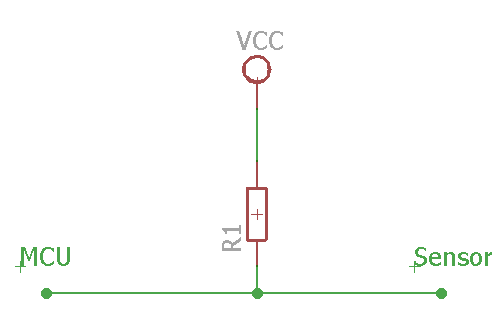
\includegraphics[width=0.8\textwidth]{figures/onewire_eksempel.png}
  \caption{1-Wire data forbindelse mellem sensor og mikroprocessor.}
  \label{one_wire_schematic}
\end{figure}

1-wire fungere lidt anderledes end en normal data forbindelse. Data bliver læst som tiden hvor der er et 0 V signal. Herfra trækker pull-op modstanden signalet høj hver gang der intet signal er. Der vil ligge 5 V på dataforbindelsen indtil enten sensor eller mikroprocessor begynder at sende 0 V, hvor den anden enhed så kan registrer hvor længe der ligge 0 V på dataforbindelsen. Tidslængden af 0 V signalet afgører om det skal opfattes som et 0 eller 1. Hvis der skal skrives et 0 udsendes der et 0 V signal i 60 $\mu$S og hvis der skal skrives 1 sendes der 0 V i 15 $\mu$S. 

Når der skal læses over 1-Wire forbindelse sker dette 30 $\mu$S efter et fald er registreret i spændingen. Dette vil så sige at da 0 svarer til et delay på 60 $\mu$S vil en spænding på 0 V måles her, og da 1 svarer til et delay på maksimum 15 $\mu$S vil en spænding på 5 V eller et højt signal aflæses her.


\begin{figure}[h!]
  \centering
  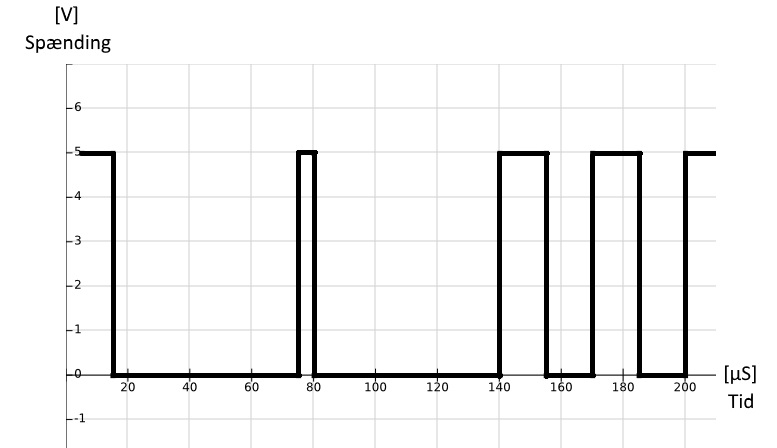
\includegraphics[width=0.8\textwidth]{figures/onewire.png}
  \caption{1-Wire graf som viser hvad der ligger på dataforbindelsen når der bliver skrevet til den.}
  \label{onewire_graph}
\end{figure}

På figur \ref{onewire_graph} ses det hvordan det vil se ud hvis man ønsker at sende et 0xC over 1-Wire forbindelsen. Det binære tal for 0xC er 1100 og da 1-Wire skriver fra LSB (least significant bit), skal det ses bagfra. Dette ses på grafen som 2 "store" mellemrum hvor der bliver skrevet 0 V på dataforbindelsen efterfulgt af to "korte" som svarer til to 1 taller. Dette er blevet eftermålt med et oscilloskop og kan ses på figur \ref{SCR01}.
\fxnote{lav LSB i glossary}

\begin{figure}[h!]
  \centering
  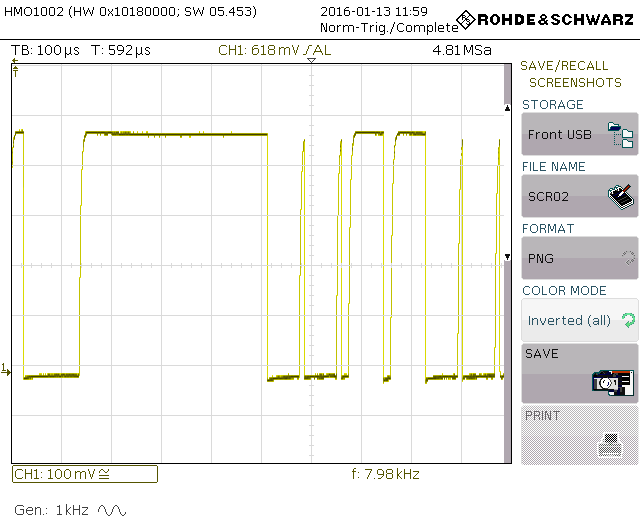
\includegraphics[width=0.8\textwidth]{figures/SCR02.png}
  \caption{Måling af 1-Wire data forbindelse med et oscilloskop.}
  \label{SCR02}
\end{figure}

Figuren viser hvad der måles på dataforbindelsen når mikroprocessoren skriver SKIPROM kommandoen til sensoren.
Fra ca. midten af figuren ses SKIPROM funktionen som består af 0xCC eller 1100 1100 i binær. Starten af 1100 (læst fra LSB) ses på i midten af grafen.


\newpage

\subsection{Overblik}
Sensoren som er beskrevet i hardwareafsnittet skal kommunikere med arduino boardet. Dette kræver nogle trin som kan findes i databladet til sensoren. På figur \ref{sensor_kom} ses et overblik over de funktioner som skal til for at aflæse sensoren. Disse funktioner er konstrueret ud fra databladet. Disse tre trin skal følges præcist for at tilgå sensoren. De tre trin er en initialisering(initialization), ROM command og function command.

I databladet til ds18b20 sensoren ses et flowchart der viser hvordan mikroprocessoren kommunikerer med sensoren og hvordan den tilgår de funktioner som sensoren kan udføre. Ud fra flowchartet har gruppen konstrueret en mindre version, som indeholder de minimale funktioner som skal anvendes for at måle temperaturændringer. Desse funktioner ses på figur \ref{sensor_kom}.



\begin{figure}[h!]
  \centering
  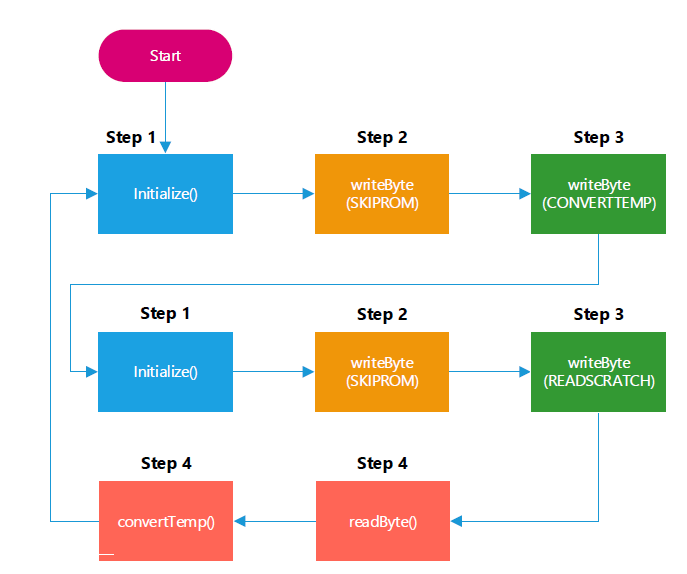
\includegraphics[width=1\textwidth]{figures/sensor_communication.png}
  \caption{Kommunikation med sensor.}
  \label{sensor_kom}
\end{figure}
\fxnote{ret størrelse til på alle billeder(noget der skal gøres til sidst!)}
\\

Navnene vist på figur \ref{sensor_kom} er de funktionsnavne der er givet i softwaren. De følger flowchartet for den mindste kommandovej der skal til for at tilgå og aflæse en temperatur måling af sensoren. Måden de er konstureret på vil blive forklaret i følgende underafsnit.

\newpage
\subsection{Initialize()}
Initialiseringsfunktionen, som ses på figur \ref{sensor_kom}, er konstrueret ved at finde intervallerne som er nødvendige for at tilgå sensoren over en 1-wire forbindelse. Disse er aflæst af en graf fra databladet (jf. figur \ref{sensor_kom}).




\begin{figure}[h!]
  \centering
  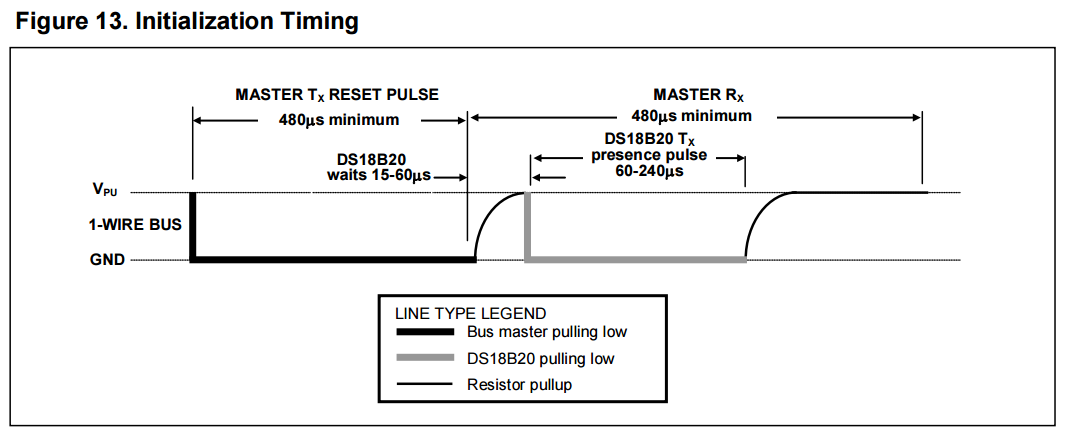
\includegraphics[width=0.5\textwidth]{figures/Initialization_timing.png}
  \caption{Illustration fra databladet som viser hvordan sensor skal initialiseres.}
  \label{sensor_kom}
\end{figure}

Fra databladet ses at 1-wire forbindelsen skal have en reset pulse i minimum 480$\mu$S og en presence pulse vil blive sendt fra sensoren til mikroprocessoren inden for 60-240$\mu$S. Dette gøres ved at sende et low signal som svare til reset pulsen. Derefter sættes forbindelsen til input, hvor den vil gå i tri-state mode og pull-up modstanden vil trække signalet højt. 
\\
\\
I koden bliver dette gjort ved at kalde digitalWrite med low som parameter, i kombination med et delay på 500$\mu$S. Derefter sættes pinMode til input og et delay på 500$\mu$S anvendes igen. Dette kan ses på figur \ref{sensor_kode}.

\begin{figure}[h!]
  \centering
  \includegraphics[width=1\textwidth]{figures/Init.png}
  \caption{Initialisering kode.}
  \label{sensor_kode}
\end{figure}

\fxnote{evt noget afslutning på dette underafsnit?}

\subsection{writeByte()}
WriteByte() er en funktion som er blevet konstrueret ud fra samme fremgangsmåde som Initialize() funktionen. Dette er gjort ved at aflæse en graf der indeholder intervaller som skal til for at tilgå sensoren.

\begin{figure}[h!]
  \centering
  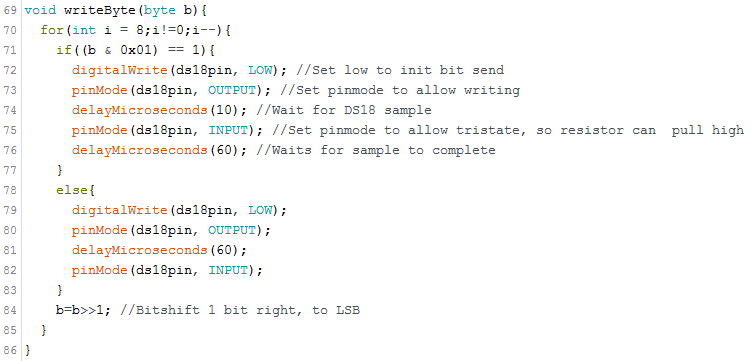
\includegraphics[width=1\textwidth]{figures/write_byte.png}
  \caption{writeByte() arduino kode.}
  \label{write_byte}
\end{figure}
\fxnote{set firkant eller noget rundt om alle vores kodeeksempler så de ikke går i et med teksten omkring}

writeByte 